The literature review introduced the vehicle routing problem and presented the available solution methods. In this chapter, we demonstrate a real-world problem of route planning in food delivery and elaborate the constraints and objectives in detail.

The objective of this work is to come up with a suitable approach for the planning of food delivery. Food delivery may involve several categories, such as recurrent meal box delivery, grocery delivery, or delivery of ingredients. In this article, the term food delivery will be used to refer to online restaurant delivery, which is a courier service in which a restaurant or a third party logistics company delivers food to a customer. This food is typically fresh (hot or cold) and is intended to be eaten right away. Therefore, the food is picked up by the driver soon after it is prepared by the restaurant. The delivery orders are typically on demand, i.e., the customers expect their food to arrive in a short period of time after placing the order. These orders are placed via restaurant websites, a phone call, or a mobile application \cite{food-delivery2020}.

The prepared food is prone to damage if dropped, tilted, or kept for a longer duration. Therefore, technology must be involved in the process of food delivery. Food portions are usually packed in plastic or paper containers which are stored in thermal bags or boxes while being carried by the courier. In addition, to reduce the duration from cooking to delivery and, consequently, to ensure customer satisfaction, software tools and planning need to be engaged \cite{food-delivery2020}.

The costs associated with the delivery service are paid either by the customer, the restaurant, or are split between both parties. These costs include drivers' salaries, gas costs, vehicle amortization, or other transportation costs. The aim of the planning procedure is to minimize those costs and consequently, increase the revenue of the service. However, in the food delivery business, customer satisfaction is commonly the most important objective, because it results in customer retention, ultimately leading to a scalable and successful business.

From the VRP perspective, food delivery has its own specifics compared to other categories of logistics. The four most important ones with respect to route planning are:
\begin{description}
    \item[Dynamicity] New information is revealed during the day, such as the arrival of new orders, unexpected delays due to traffic, or changing the number of drivers. Therefore, high emphasis is placed on the speed of the selected algorithm, as the drivers need to react to changes as quickly as possible.
    \item[Short Time Windows] Customers expect their food to arrive shortly after they order it. In addition, ready-to-eat food has short lastingness and needs to be delivered as soon as possible to secure its quality.
    \item[Soft Time Window Constraints] The time windows for food delivery are generally soft, meaning they can be violated carrying a penalty cost. In addition, visiting a customer before the specified time window is usually preferred over being late, so the penalty is lower in that case.
    \item[Peak Times] Food delivery has peak times around lunchtime and dinnertime. With this, the number of required drivers need to change dynamically according to the time of the day.
\end{description}
    
\section{Formal Definition}
    
    It is clear that in the context of food delivery, each customer request consists of transporting goods (food) from one pickup location to one drop-off location. As there may be more restaurants preparing food, rather than a single depot, it is the case of \textit{pickup and delivery problem} (PDP). Since food delivery commonly involves multiple drivers and time window constraints, the ultimate generalization of this problem can be referred to as the \textit{pickup and delivery problem with time windows} (PDPTW). This variant also involves capacity constraints, i.e., how many food portions can each driver carry at any moment. In addition, one feature that is required for our use case is that the drivers can start at arbitrary locations rather than a single depot. An example of a single request is shown in figure \ref{fig:example-request}.
    
    \begin{figure}[!ht]
        \centering
        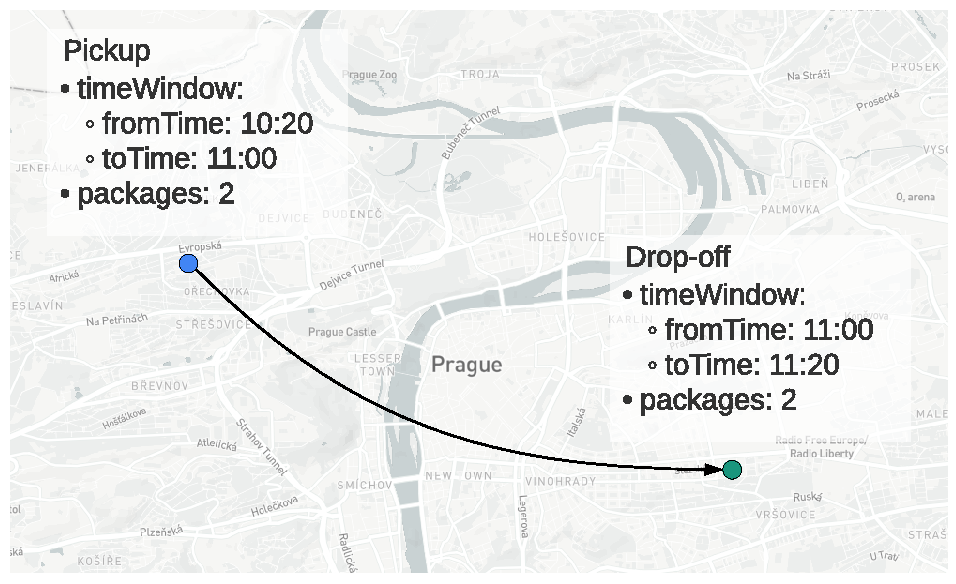
\includegraphics[width=0.8\textwidth]{figures/example-request.pdf}
        \caption{An example of a single request.}
        \label{fig:example-request}
    \end{figure}
    
    Using a similar notation to Cordeau (2006) \cite{cordeau}, let us define this problem formally:
    
    We are given a complete graph $G = (V,A)$, where $V$ is the set of nodes and $A = \{(i,j) : i,j \in V, i \neq j \}$ is the set of arcs. $V$ is further partitioned into three subsets $V = S \cup P \cup D$. The set $S, |S| = k$ is the set of start/depot nodes, i.e., the nodes where the couriers/drivers $K = {1,\cdots,k}$ are initially located. The positive integer $k$ is the number of couriers/drivers for which the routes are computed. The set $P$ is the set of pickup nodes $P = \{1,\cdots,p\}$, where $p$ is the number of pickup nodes, and $D$ the set of drop-off nodes $D = \{1,\cdots,d\}$, where $d$ is the number of drop-off nodes.
    
    It holds that $d \geq p$ as there must be at least the same number of drop-off nodes as pickup nodes. There may be more drop-off nodes then pickup nodes as the planning phase runs in a dynamic environment, and thus some packages can be already picked up when the planning process is called. This will be further explained in section \ref{sec:dynamicity}.
    
    There are two types of requests $r \in R$, where each request $r$ is a pair of nodes from $V$. It is either a full request $r^{\mathrm{full}}_{i,j}$ which consists of transporting a package from the pickup node $i \in P$ to the delivery node $j \in D$, or a partial request $r^{\mathrm{partial}}_{k,i}$ which consists of delivering an already picked up package by the driver $k \in K$ to the drop-off node $i \in D$.
    
    A nonnegative pickup/drop-off service time $t^{\mathrm{service}}_i$ is associated with every node $i \in V$, which denotes the required time the driver needs to spend at node $i$. It is assumed that $t^{\mathrm{service}}_i = 0\;\forall i \in S$. A time window $w_i = [w^s_i, w^e_i]$ is associated with each node $i \in V$, where $w^s_i$ is the start of the time window and $w^e_i$ is the end of the time window. It is assumed that $w_i = (-\inf, \inf)\;\forall i \in S$. Finally, a travel time $t^{\mathrm{travel}}_{i,j}$ and distance $m_{i,j}$ are associated with each pair of vertices $(i, j) \in A$. If a driver location is not known in advance, we assign $t^{\mathrm{travel}}_{k,i} = $ 15 min and $m_{k,i} = $ 10 km for the driver $k$, assuming that it takes approximately 15 minutes and 10 kilometers to travel from a random location to another random location in the city.
    
    Additionally, the capacity constraints are defined for the vehicles. Each driver $k \in K$ has a capacity $c_k \in \mathbb{N}$. Also, a demand $d_i \in \mathbb{Z}$ is assosiated with each node $i \in V$, and denotes how much of the capacity is utilized when completing service at node $i$. It holds that $d_i > 0\,\forall i \in P$ and $d_i < 0\,\forall i \in D$.
    
    The output of the algorithm is a set of routes $E = \{e_0,\cdots,e_k\}$, where $k$ is the number of drivers and the route $e_l$ for each driver $l \in K$ is sequence of nodes $i \in V$ such that each route starts with a start node $l \in S$, where the driver is initially located. It also holds that for each full request $r^{\mathrm{full}}_{i,j}$, pickup node $i$ and drop-off node $j$ are in the same route $e$, and node $i$ precedes $j$ in route $e$. Similarly, for each partial request $r^{\mathrm{partial}}_{l,i}$ it holds that the drop-off node $i$ is in route $l$, corresponding to driver $l$. For each node $i$ in route $e$ an estimated time of arrival $t^{\mathrm{eta}}_i$ and an estimated time of departure $t^{\mathrm{etd}}_i$ are associated, where $t^{\mathrm{etd}}_i \geq t^{\mathrm{eta}}_i + t^{\mathrm{service}}_i$. Additionally, for the solution to be feasible, at any node, the driver cannot exceed its capacity, i.e., for each route $e_l$ it must hold $\sum_{i = 1}^{u} d_i \leq c_l\; \forall u \in \{1,\ldots,|e_l|\}$
    
    It is not guaranteed that a plan which satisfies all time window constrains always exists. Therefore, the time window constrains are considered soft, meaning they can be violated carrying a penalty cost.
    
    There are two objectives to this problem. First, to minimize the deviation from the specified time windows: \[\min\;\sum_{i \in V}\;\max(w^s_i - t^{\mathrm{eta}}_i, t^{\mathrm{eta}}_i - w^e_i)\]
    Second, to minimize the total distance travelled by the drivers: \[\min\;\sum_{e \in E}\;\sum_{i = 0}^{|e|-1}m_{i,i+1}\]The first objective provides for customer satisfaction, the other contributes to reducing the costs associated with the delivery.

    \subsection{Dynamicity} \label{sec:dynamicity}
    
    Online food delivery planning is a dynamic VRP as described in section \ref{sec:dynamic}. As new information is revealed during the planning horizon, this information needs to be incorporated into existing plans as soon as possible, so the drivers are able to react to this information. Most studies in this field consider new pieces of information as the events that trigger the replanning process \cite{darp-survey}. Typically, the planning process should not take more than 2 minutes. Therefore, a strong emphasis is placed on the time complexity of the planning algorithm. Some of the events that trigger the replanning procedure are the following:
    
    \begin{description}
      \item [A new delivery order is placed] When a customer makes an order, the pickup and drop-off nodes need to be incorporated into one of the existing plans.
      \item [The number of drivers changes] When an existing driver goes off duty, we need to make sure that his assigned deliveries will be taken care of by someone else. Similarly, when a new driver goes on duty, he gets some deliveries that have already been assigned to his colleagues.
      \item [A driver is delayed] The time estimates are never exact, and it may happen that a driver encounters a problem that causes his delay. In that case, some of the deliveries assigned to him should be handed to other drivers to compensate for the delay. The replanning procedure is triggered if the accumulated delay $d > d^{\mathrm{lim}}$, where $d^{\mathrm{lim}}$ is the threshold.
    \end{description}
    
    Because the plans need to be recomputed in real time, it often happens that by the time the planning occurs, some packages have already been picked up by some of the couriers. In that case, we need to make sure that only the drop-off nodes are provided to the planning process and that the correct drivers will be handling them.
    
    Another issue comes from the asynchronicity of planning. The planning procedure always takes the current state, i.e., the information it currently has, and takes some time to produce a solution. By the time the planning procedure ends, the current state may change, for example, some deliveries were picked up, another delivery was dropped off, a driver went off-duty, or a new delivery order arrived. When such a situation occurs, the planning procedure must react to these changes by either resolving those inconsistencies, or by rerunning the replanning procedure again.

\section{Broader Context within GoDeliver}

    \emph{GoDeliver}\footnote{\url{https://godeliver.co/}} is a software solution for governing deliveries developed by Cognitic\footnote{\url{https://cognitic.ai/}} with the aim of making the city logistics simpler and more efficient. It provides clients with everything they need for managing their own fleet of drivers, including the driver application, real-time monitoring, automatic dispatch, and route planning. Figure \ref{fig:dashboard} shows the driver application and the real-time tracking dashboard.
    
    \begin{figure}[!ht]
    	\centering
    	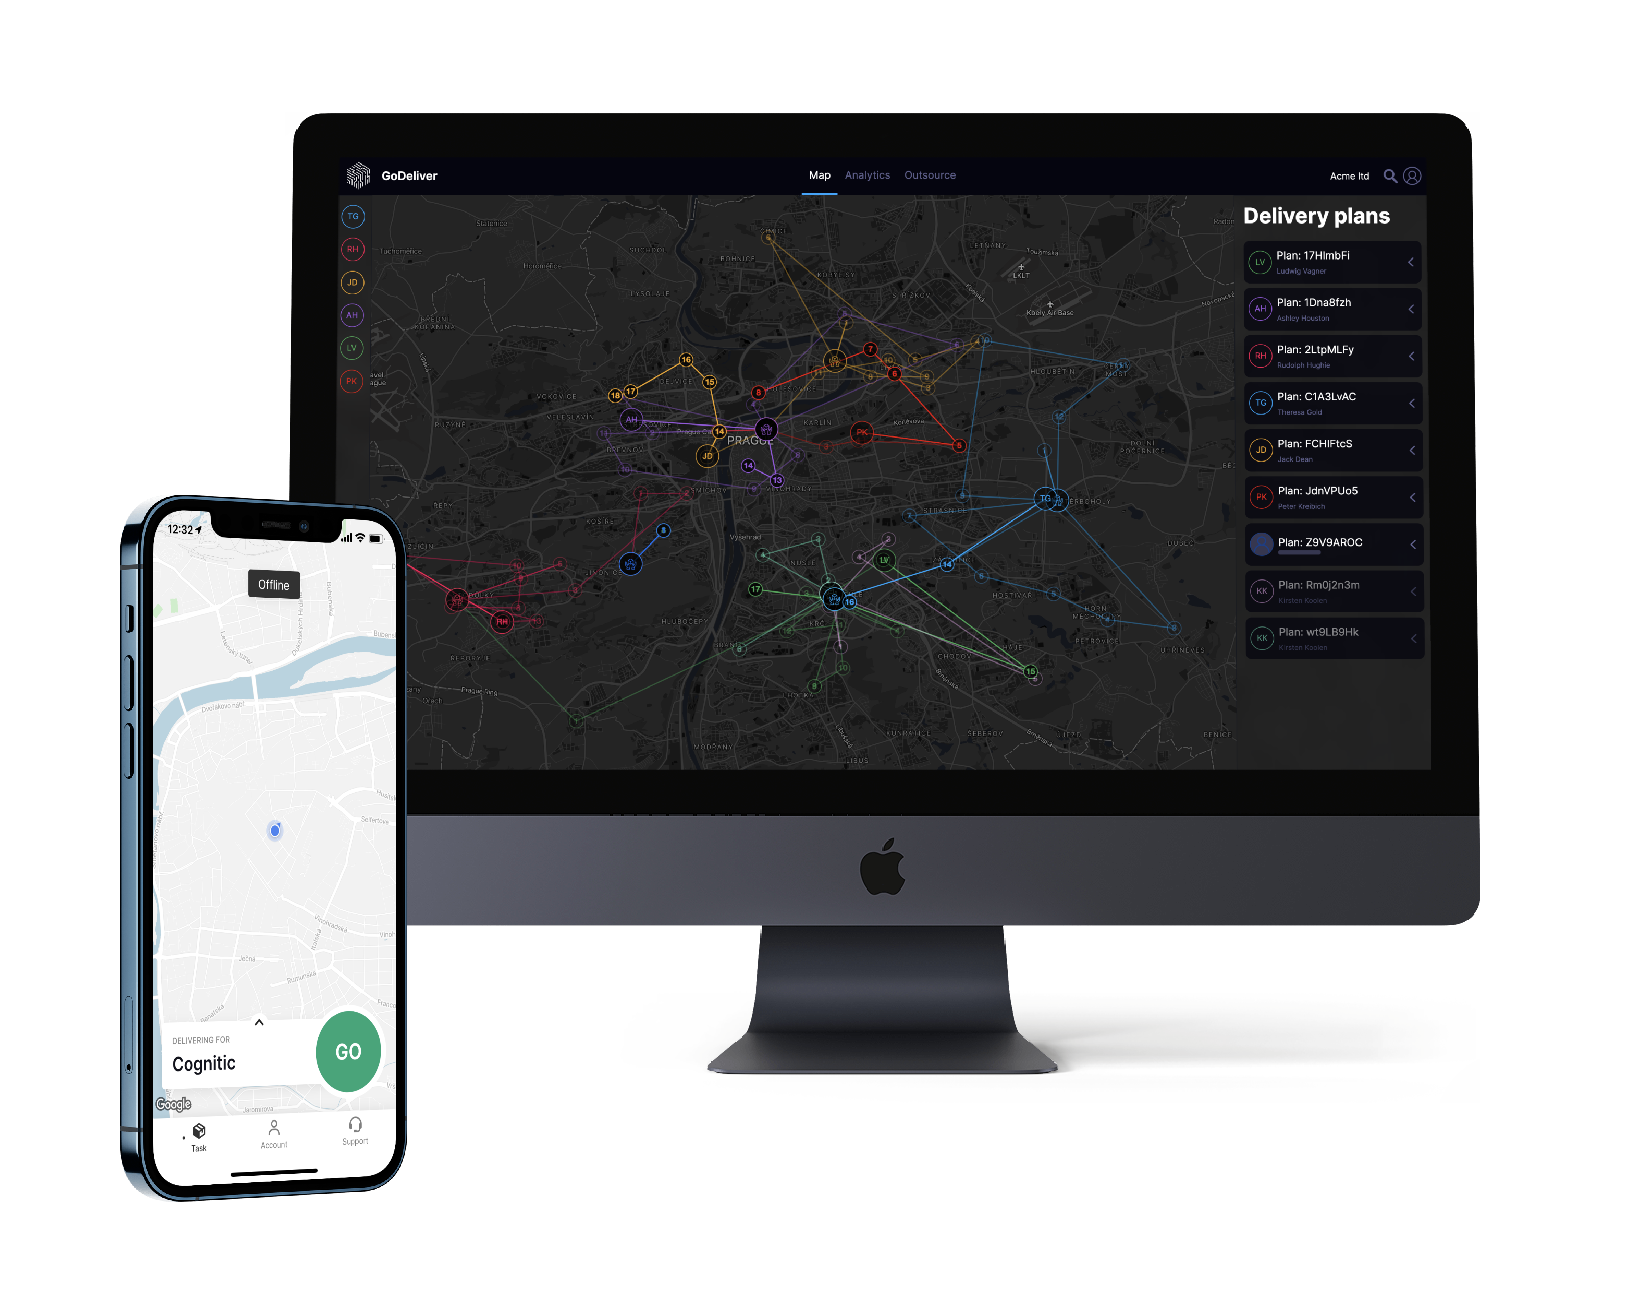
\includegraphics[width=0.8\textwidth]{figures/godeliver-system.pdf}
    	\caption[GoDeliver driver application and real-time tracking dashboard]{GoDeliver driver application and real-time tracking dashboard}
    	\label{fig:dashboard}
    \end{figure}

    \subsection{Features}

    	The most important features that GoDeliver provides are:
    	\begin{description}
    		
    		\item [Driver Management] The mobile application available for \emph{iOS} and \emph{Android} is used to provide information to drivers about their tasks. It shows the address of the next pickup or drop-off location along with the options to open the navigation and to call the customer. The application tracks the driver's location and sends information about completed tasks to the GoDeliver backend.
    		
    		\item [Real-time Visualization] The tracking dashboard for dispatchers and logistics managers allows to visualize deliveries, drivers, and routes, along with the estimated arrival times and delays.
    		
    		\item [Route Optimization] Probably the most critical feature of GoDeliver is the automated route planning. This is essentially the VRP solver which supports different VRP variants, depending on the customer's needs.
    		
    		\item [Automatic Dispatch] The aim of GoDeliver is to eliminate the need for human dispatchers assigning tasks to individual drivers. Therefore, automatic dispatch is a mechanism designed to tackle dynamic scenarios, where the system needs to react to new information, such as receiving or cancelling orders, changing the number of drivers, or route accidents and delays.
    	
    		\item [Customer Tracking] To ensure the best possible experience for the end customers, GoDeliver offers order tracking. This web app is sent to users via SMS message or email and shows the status of their order and the current location of the driver.
    		
    		\item [Data Visualisation] GoDeliver enables data-driven decisions by gathering and visualising data about the logistics fleet, such as delays, compound delivery costs, and other statistics.
    		
    		\item [External Integrations] To integrate GoDeliver within existing systems, the software provides a well-documented API and plugins to popular point-of-sale systems.
            
    	\end{description}


    \subsection{Architecture} \label{sec:godeliver-current-state}
    
    A simplified architecture of GoDeliver system is shown in figure \ref{fig:godeliver-architecture-old}. The  main logic behind GoDeliver is implemented in the \emph{Backend Service}. This service is a server application that communicates with the tracking dashboard and driver applications via a REST API. It also provides public endpoints for integrating with other systems. The data are stored in a Firestore Database\footnote{\url{https://firebase.google.com/docs/firestore}}. On certain events that should trigger the replanning a new Celery\footnote{\url{https://docs.celeryproject.org/}} job is created. The \emph{Replan Runner} consumes these jobs, calls the \emph{Logistics Planner} (highlighted in yellow color), and writes the produced solution to the database.
    
    The Logistics Planner is a stateless server that provides a single endpoint for planning. This endpoint consumes the instance of the VRP and produces a solution. In case that the solution cannot be found, an error is returned. To obtain the real distance and travel duration between each pair of nodes, the \emph{Planning Engine} is used. This server runs our own instance of Open Source Routing Machine (OSRM)\footnote{\url{http://project-osrm.org/}} which finds the shortest paths between two pairs of coordinates. This engine works over the Open Street Map\footnote{\url{https://www.openstreetmap.org/}} data that are regularly updated to include new routes and recent closures.
    
    The Logistics Planner internally uses Google ORTools for solving the VRP instance. As mentioned in section \ref{solvers}, ORTools is unable to solve larger instances and is thus insufficient for real-world use cases. Therefore, this thesis aims to upgrade the planning algorithm to comply with the real-world applications.

    \begin{figure}[ht]
        \centering
        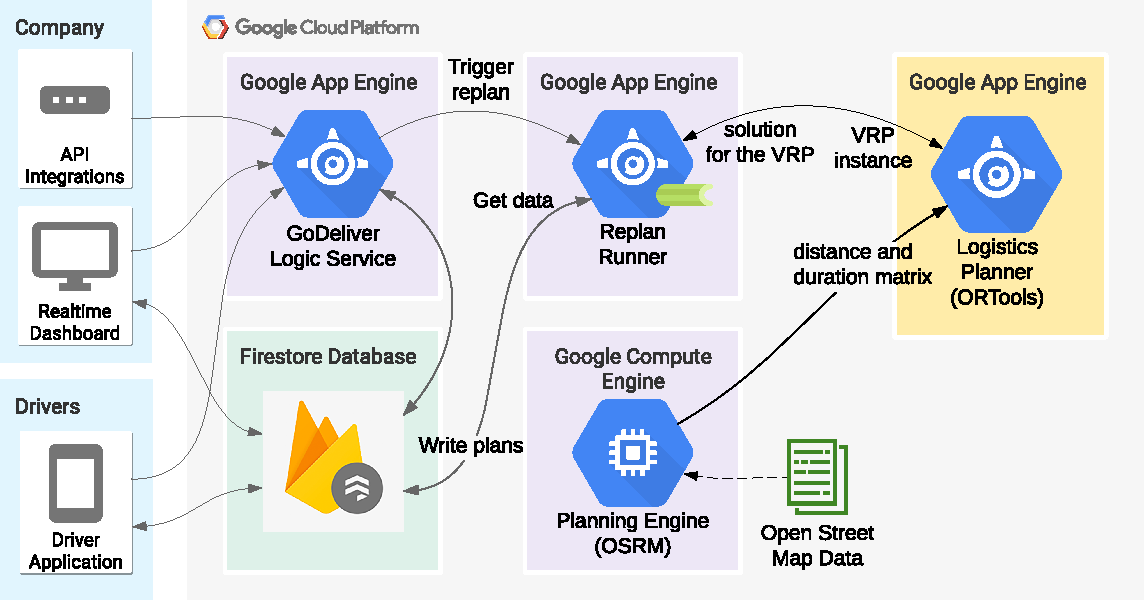
\includegraphics[width=1\textwidth]{figures/godeliver-architecture-old.pdf}
        \caption{Current state of GoDeliver architecture}
        \label{fig:godeliver-architecture-old}
    \end{figure}
